% !TeX root = ../main.tex
% \graphicspath{ {./images/} }
\section{Model}

\subsection{Overview}

To reach the objective of our research, we design a prediction model shown in Fig. 1. The input sequence is a series of data, including attributes of a video, popularity of a video under the defined time scale, and channel attributes of each observed brand. Encoder layer is used to structure the patterns of input features after feature engineering processing. Prediction layer would output a sequence of predicted popularity of given video content in future timestamps.

\begin{figure}[h]
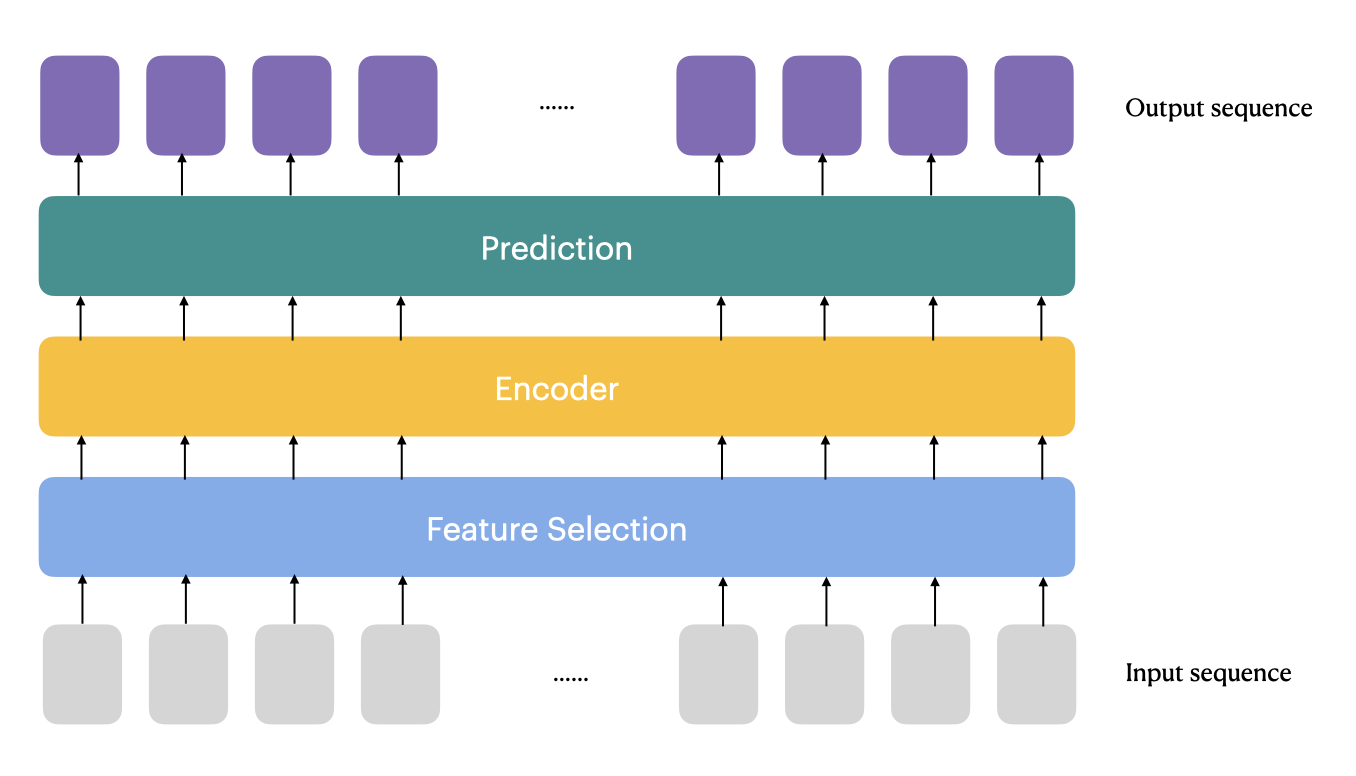
\includegraphics[scale=0.3]{figures/Proposed Model.png}
\caption{Overall framework of our proposed prediction model}
\end{figure}